% ============================================================
%  MediPilot — Accenture Innovation Challenge 2026
%  Technical White Paper | Team 01 BIT
%  Aditya Onam · Aditya Gupta · Varada Patel
% ============================================================
\documentclass[10pt,a4paper,twocolumn]{article}

\usepackage[T1]{fontenc}
\usepackage[utf8]{inputenc}
\usepackage{newtxtext,newtxmath}
\usepackage{helvet}
\usepackage{microtype}

% ---------- Palette ----------
\usepackage[table,svgnames]{xcolor}
\definecolor{AccPurple}{HTML}{A100FF}
\definecolor{SecPurple}{HTML}{6F00B8}
\definecolor{DeepPurple}{HTML}{4B0082}
\definecolor{DarkPlum}{HTML}{24003D}
\definecolor{NearBlack}{HTML}{111111}
\definecolor{MedGray}{HTML}{666666}
\definecolor{CardBg}{HTML}{F7F7F7}
\definecolor{SoftGray}{HTML}{F2F2F2}
\definecolor{Border}{HTML}{E2E2E2}
\definecolor{White}{HTML}{FFFFFF}
% clinical accents — used only as ATP colour-band identifiers
\definecolor{TriRed}{HTML}{C0392B}
\definecolor{TriAmber}{HTML}{C98A17}
\definecolor{TriGreen}{HTML}{2E7D5B}

\usepackage[a4paper,top=1.9cm,bottom=2.0cm,left=1.8cm,right=1.8cm]{geometry}
\setlength{\columnsep}{0.72cm}

\usepackage{graphicx}
\usepackage{booktabs,array}
\usepackage{enumitem}
\usepackage[most]{tcolorbox}
\usepackage{titlesec}
\usepackage{fancyhdr}
\usepackage{lastpage}
\usepackage{caption}
\usepackage{tikz}
\usetikzlibrary{positioning,calc,arrows.meta,fit,backgrounds}
\usepackage[colorlinks=true,linkcolor=SecPurple,urlcolor=SecPurple,citecolor=SecPurple,
  pdftitle={MediPilot: Asymmetric-Autonomy AI for Continuous ED Re-Triage},
  pdfauthor={Aditya Onam, Aditya Gupta, Varada Patel}]{hyperref}

% ---------- Text colour + spacing ----------
\color{NearBlack}
\setlength{\parindent}{1em}
\setlength{\parskip}{0pt}
\linespread{1.02}
\raggedbottom
% keep floats from crowding text out of a column
\renewcommand{\topfraction}{0.92}
\renewcommand{\textfraction}{0.06}
\renewcommand{\floatpagefraction}{0.80}
\setlength{\textfloatsep}{10pt plus 2pt minus 2pt}
\setlength{\dblfloatsep}{10pt plus 2pt minus 2pt}
\setlength{\dbltextfloatsep}{10pt plus 2pt minus 2pt}

% ---------- Headings ----------
\titleformat{\section}{\sffamily\bfseries\small\color{NearBlack}}
  {\textcolor{AccPurple}{\thesection}}{0.5em}{\MakeUppercase}
  [\vspace{-4pt}\textcolor{AccPurple}{\rule{\linewidth}{1pt}}]
\titlespacing*{\section}{0pt}{9pt}{4pt}
\titleformat{\subsection}{\sffamily\bfseries\footnotesize\color{SecPurple}}
  {\thesubsection}{0.5em}{}
\titlespacing*{\subsection}{0pt}{7pt}{2pt}

% ---------- Boxes ----------
\tcbset{mpbox/.style={enhanced,sharp corners=all,
  colback=CardBg,colframe=AccPurple,boxrule=0pt,leftrule=2.2pt,
  left=5pt,right=5pt,top=4pt,bottom=4pt,
  fontupper=\footnotesize}}
\tcbset{mpthesis/.style={enhanced,arc=2pt,
  colback=DarkPlum,colframe=DarkPlum,coltext=White,boxrule=0pt,
  left=6pt,right=6pt,top=5pt,bottom=5pt,fontupper=\footnotesize}}
\tcbset{mpcode/.style={enhanced,arc=1pt,
  colback=NearBlack,coltext=White,colframe=NearBlack,boxrule=0pt,
  left=5pt,right=5pt,top=4pt,bottom=4pt,
  fontupper=\ttfamily\scriptsize}}

\setlist[itemize]{leftmargin=1.1em,topsep=2pt,itemsep=1pt,parsep=0pt,
  label={\footnotesize\textcolor{AccPurple}{\textbullet}}}
\setlist[enumerate]{leftmargin=1.4em,topsep=2pt,itemsep=1pt,parsep=0pt}

\captionsetup{font={footnotesize,sf,color=MedGray},
  labelfont={bf,color=AccPurple},labelsep=period,skip=4pt}

% ---------- Page furniture ----------
\pagestyle{fancy}\fancyhf{}\renewcommand{\headrulewidth}{0pt}
\fancyfoot[C]{\textcolor{Border}{\rule{\linewidth}{0.4pt}}\\[2pt]
  \sffamily\scriptsize\color{MedGray}%
  MediPilot \textbullet\ Team 01 BIT\hfill
  \textcolor{AccPurple}{\thepage}\,/\,\pageref{LastPage}}

% ---------- TikZ styles ----------
\tikzset{
  bx/.style={draw=Border,fill=CardBg,rounded corners=1.6pt,inner xsep=4pt,
    inner ysep=3pt,align=left,font=\sffamily\tiny,text=NearBlack},
  bxa/.style={bx,fill=AccPurple!7,draw=AccPurple!40},
  bxd/.style={bx,fill=DarkPlum,draw=DarkPlum,text=White},
  flow/.style={-{Latex[length=1.3mm,width=1mm]},draw=SecPurple,line width=0.45pt},
  loop/.style={-{Latex[length=1.3mm,width=1mm]},draw=AccPurple,line width=0.45pt,
    dash pattern=on 1.3pt off 1.3pt},
  tg/.style={font=\sffamily\bfseries\tiny,text=AccPurple},
  lbl/.style={font=\sffamily\tiny,text=MedGray},
}
\newcommand{\ly}[2]{{\bfseries\textcolor{AccPurple}{#1}}\;\;{\bfseries #2}}
\newcommand{\lyo}[1]{{\bfseries #1}}                      % no tag
\newcommand{\sub}[1]{\\[1pt]{\color{MedGray}#1}}
\newcommand{\subw}[1]{\\[1pt]{\color{AccPurple!14!white}#1}}  % on dark plum

\begin{document}

% ======================= TITLE BLOCK =======================
\twocolumn[{%
\vspace{-6mm}
\noindent\begin{minipage}[b]{0.74\textwidth}
  \raggedright\hyphenpenalty=10000\exhyphenpenalty=10000
  {\sffamily\scriptsize\color{AccPurple}\bfseries
   ACCENTURE INNOVATION CHALLENGE 2026 \ \textbullet\ \ ROUND I \ \textbullet\ \ PATIENTTRIAGE.AI}\\[5pt]
  {\sffamily\bfseries\LARGE\color{NearBlack}
   \textcolor{AccPurple}{Medi}Pilot: Asymmetric-Autonomy AI for\\[2pt]
   Continuous Re-Triage in the Indian ED}
\end{minipage}\hfill
\begin{minipage}[b]{0.24\textwidth}
  \raggedleft
\includegraphics[height=22pt]{assets/accenture_logo.png}
\end{minipage}

\vspace{5pt}
\noindent\textcolor{AccPurple}{\rule{\textwidth}{1.4pt}}\\[-3pt]
\noindent\textcolor{Border}{\rule{\textwidth}{0.5pt}}

\vspace{5pt}
\noindent{\sffamily\footnotesize\bfseries
  Aditya Onam \quad Aditya Gupta \quad Varada Patel}\\[1pt]
\noindent{\sffamily\scriptsize\color{MedGray}
  Team 01 BIT \ \textbullet\ \ Indian Institute of Technology Patna \ \textbullet\ \ August 2026}

\vspace{7pt}
\begin{tcolorbox}[mpbox,colback=White,leftrule=0pt,left=0pt,right=0pt,top=2pt,bottom=2pt]
{\sffamily\scriptsize\bfseries\color{AccPurple}ABSTRACT}\\[2pt]
\footnotesize
Emergency department (ED) crowding kills through a structural defect, not through
individual error: acuity is assigned once, at arrival, and the queue that results is
static while the patient's physiology is not. Emergency Severity Index mistriage
affects 32.2\% of US ED visits, and India had no nationally standardised ED triage
protocol before the AIIMS Triage Protocol (ATP). We present \emph{MediPilot}, a
continuous re-triage platform built on a single architectural invariant:
\textbf{the system may raise a waiting patient's priority autonomously and may never
lower it below a human-assigned level}. Escalation costs one nurse assessment;
de-escalation can cost a life, so it stays with a human. We show how this invariant
propagates into every layer --- outcome-derived rather than nurse-imitating labels,
leakage control enforced mechanically in CI after the Epic Sepsis Model's failure
(AUC 0.63, sensitivity 33\%), an LLM restricted by output grammar to perception,
conformal abstention rather than silent guessing, and a five-minute re-scoring cycle
that is both the primary safety mechanism and the commercial wedge. We specify the
data acquisition path, training methodology, evaluation protocol
(under-triage at fixed over-triage; equalised false-negative rate; stepped-wedge
causal attribution), tiered edge deployment at a target of under Rs.\,5 per
encounter, and the CDSCO/ICMR/DPDP compliance route --- including the gap where
ABDM consent does not by itself satisfy DPDP Act 2023 for model-input use.

\vspace{3pt}
{\sffamily\scriptsize\color{MedGray}\textbf{\color{NearBlack}Keywords:}\;
clinical decision support \textbullet\ emergency triage \textbullet\ asymmetric cost
learning \textbullet\ conformal prediction \textbullet\ federated learning
\textbullet\ SaMD regulation \textbullet\ Indian healthcare}
\end{tcolorbox}
\vspace{4pt}
}]

% ======================= 1. INTRODUCTION =======================
\section{Introduction}

The danger of an ED waiting room is not that patients arrive critically ill; it is
that they \emph{become} critically ill after being assigned a low priority, and no
mechanism exists to notice. A patient with mild chest discomfort receives a Yellow
designation and sits down. Twenty minutes later they are hemodynamically unstable.
The triage nurse is by then registering three new arrivals. The patient
deteriorates unseen.

This is the \textbf{single-point assessment model}, and it is a property of the
process rather than of any clinician within it. Its failure rate is measurable:
\textbf{32.2\%} of total US ED visits are affected by ESI mistriage
[9]. In India the position was worse until recently --- no evidence-based
national triage standard existed before the AIIMS Triage Protocol, a three-tier
Red/Yellow/Green system since adopted by AIIMS Bhubaneswar, CMC Vellore, GTB Delhi
and the Kerala DHS [3]. Most Indian EDs are staffed by general
practitioners or residents without formal emergency-medicine training [2],
so any workable system must run in a district hospital with one physician and one
nurse as reliably as in a tertiary centre.

\textbf{Contributions.} (i) A decision-theoretic autonomy boundary --- autonomous
escalation, never autonomous de-escalation --- and its propagation as a hard
constraint through six architectural layers (\S\ref{sec:principle}--\S\ref{sec:arch}).
(ii) A label and feature design that avoids both nurse-label imitation and the
target-leakage failure that broke the Epic Sepsis Model, with leakage enforced by
CI rather than by policy (\S\ref{sec:prior}, \S\ref{sec:data}).
(iii) An evaluation and rollout protocol whose primary metric is under-triage at
fixed over-triage, with fairness defined as equalised false-negative rate
(\S\ref{sec:eval}).
(iv) A deployment and governance path specific to Indian infrastructure and
regulation (\S\ref{sec:deploy}).

% ======================= 2. PRIOR FAILURE =======================
\section{Why Prior Clinical AI Failed}
\label{sec:prior}

Wong et al.\ [12] externally validated the Epic Sepsis Model across
38{,}455 hospitalisations at the University of Michigan (Dec 2018--Oct 2019).
The model was already deployed at hundreds of US hospitals.

\begin{center}\footnotesize\sffamily
\begin{tabular}{@{}lcccc@{}}
\toprule
\rowcolor{AccPurple!10}
\textbf{ESM (external)} & AUC & Sens. & Spec. & PPV\\
\midrule
Reported performance & \textcolor{AccPurple}{\bfseries 0.63} & 33\% & 83\% & 12\%\\
\bottomrule
\end{tabular}
\end{center}
\vspace{-2pt}
{\footnotesize\color{MedGray}Two-thirds of sepsis cases missed; 109 alerts raised per
true positive found.}

\vspace{4pt}
The root cause was \textbf{target leakage}: the model used antibiotic-order timing as
an input feature. It therefore detected \emph{clinician suspicion} rather than the
underlying physiology --- it learned to imitate the process it was meant to augment,
and failed exactly where that process was already failing.

\begin{tcolorbox}[mpbox]
\textbf{Structural response.} MediPilot maintains a \textbf{temporal feature
registry} recording, per feature, its earliest availability time, source system and
leakage class (\texttt{SAFE} / \texttt{CONDITIONAL} / \texttt{PROHIBITED}). Any
feature downstream of clinician suspicion is \texttt{PROHIBITED}, and an
\textbf{automated leakage lint} in CI fails the build if one appears in a training
feature set. Inclusion is mechanically impossible, not procedurally discouraged
(\S\ref{sec:data}).
\end{tcolorbox}

A second precedent constrains the language model. Haim et al.\ [6] found
GPT-4 systematically miscalibrated against trained clinical raters, with a documented
tendency to \emph{overestimate} severity. MediPilot therefore gives the LLM no
production rule for acuity at all (\S\ref{sec:arch}).

% ======================= 3. PRINCIPLE =======================
\section{The Asymmetric Autonomy Principle}
\label{sec:principle}

\begin{tcolorbox}[mpthesis]
\itshape MediPilot may escalate a waiting patient's queue position autonomously.
It may never de-escalate a patient below a human-assigned level autonomously.
\end{tcolorbox}

\vspace{3pt}
This is the correct answer to an asymmetric cost structure, not a policy preference.
An unwarranted escalation (Yellow$\rightarrow$Red on a stable patient) costs one brief
nurse assessment and causes no patient harm. An unwarranted de-escalation
(Red$\rightarrow$Yellow on an evolving STEMI) costs death or permanent disability.

Let $p$ be the calibrated probability of a 24-hour critical event and let
$R = c_{\text{FN}}/c_{\text{FP}}$ be the site's miss-to-false-alarm cost ratio.
Escalation is optimal when $c_{\text{FN}}\,p \ge c_{\text{FP}}(1-p)$, giving the
operating threshold
\[
  p^{*} \;=\; \frac{c_{\text{FP}}}{c_{\text{FP}}+c_{\text{FN}}} \;=\; \frac{1}{1+R}.
\]
With $R=500$ (tertiary centre), $p^{*}\approx0.002$; with $R=100$ (district
hospital), $p^{*}\approx0.010$. $R$ is a \textbf{per-hospital configurable
parameter} set by clinical leadership at deployment and reviewed at each federated
update cycle --- it is not a global constant chosen by the vendor.

The same ratio enters training as an asymmetric loss (\S\ref{sec:train}), so the
threshold and the objective agree rather than being reconciled after the fact.

% ======================= 4. ARCHITECTURE =======================
\section{System Architecture}
\label{sec:arch}

MediPilot is a six-layer pipeline (Fig.~\ref{fig:arch}) closed by two feedback loops.

\subsection{L0 --- Capture and the feature registry}
Data arrives in three windows with sharply different availability (Fig.~\ref{fig:timeline}).
Every field is registered with its earliest availability time and leakage class
before it can be used. \textbf{Operational context} --- census, boarding count, staff
on shift, bed and ventilator availability --- is ingested by the routing layer L4
\emph{only}, and is explicitly excluded from the risk layers L2--L3, so physiologic
risk is never a function of how busy the department is.

\subsection{L1 --- The LLM structurer, perception only}
Audio $\xrightarrow{\text{IndicWhisper INT8 ASR}}$ tokens
$\xrightarrow{\text{grammar-constrained decoding}}$ SNOMED-mapped schema fields.
The output grammar \textbf{contains no production rule} for a free-text diagnosis or
an acuity recommendation, so the failure mode reported by Haim et al.\ cannot be
expressed. The nurse speaks normally; the system fills the form and reads the vitals
back for correction before committing.

\subsection{L2 --- Risk backbone, late fusion, three heads}
\begin{itemize}
  \item \textbf{GBDT} (XGBoost/LightGBM) over tabular T0--T1 fields: 100\% of
        patients, millisecond latency, native missing-value handling.
  \item \textbf{GRU / small transformer} over irregular serial vitals --- this is the
        \emph{deterioration-while-waiting} signal, invisible to any snapshot model.
  \item \textbf{Multilingual IndicBERT} over chief complaint and nurse narrative.
\end{itemize}
For ABHA-linked patients a self-supervised next-event transformer (ETHOS/CLMBR-style)
adds a history embedding. \textbf{Train-time modality dropout} forces usable estimates
from any subset, because missing data is the default case in an Indian ED, not the
exception.

\subsection{L3 --- Calibration, uncertainty, abstention}
An overconfident wrong prediction is more dangerous than an uncertain correct one.
\textbf{Per-site isotonic/Platt calibration} makes outputs interpretable as local
frequencies. \textbf{Split conformal prediction} ($\alpha=0.10$) returns an
\emph{acuity set} with a formal $\ge 90\%$ coverage guarantee instead of a spuriously
precise point estimate; \textbf{Mondrian conformal prediction} holds that coverage
separately within each demographic and linguistic subgroup. An \textbf{OOD abstention
gate} routes unfamiliar patients to manual nurse assessment with an explanatory note.
Abstention is visible, never silent.

\subsection{L4 --- Decision and routing}
L4 solves a constrained assignment problem: maximise expected clinical value subject
to hard rules no optimiser component may override.
\begin{itemize}
  \item A Red patient is never queued behind a Green patient under any resource state.
  \item Suspected STEMI routes to the cath lab regardless of throughput impact.
  \item A normal SpO\textsubscript{2} reading \textbf{alone} is never grounds for
        downward queue movement (see box below).
\end{itemize}
Bandit/RL components act only on the soft dimension --- which of several equally safe
rooms --- inside a runtime safety filter that rejects protocol-violating actions.
\textbf{Mass-casualty mode}, which switches the objective from individual
expected-value to resource-constrained population benefit, is activated only by an
authenticated senior clinician. The system never concludes on its own that a
mass-casualty event exists.

\begin{tcolorbox}[mpbox,colframe=DeepPurple]
\textbf{Pulse-oximetry bias --- a non-overridable rule.} Sjoding et al.\
[11] found occult hypoxemia in \textbf{11.7\%} of Black versus
\textbf{3.6\%} of White patients (single centre), and \textbf{17\%} versus
\textbf{6.2\%} in a multicentre VA cohort. A normal SpO\textsubscript{2} therefore
carries no de-escalation authority in L4. The ambient pallor module is calibrated
per Fitzpatrick stratum with false-negative-rate equalisation across strata.
\end{tcolorbox}

\subsection{L5 --- Presentation: one card}
The nurse sees a recommended acuity level, the \textbf{two strongest supporting
factors, one opposing factor}, and a confidence band. The opposing factor is a
deliberate falsification target: it forces engagement with reasoning rather than with
a number, which is the standard defence against automation bias. Accept or override
is one touch; an override requires a stated reason. No acuity level is ever spoken
aloud within patient earshot, and the hall speaker calls token numbers only.

\subsection{Feedback loops}
\textbf{Loop A (5 min).} Every waiting patient is re-scored. A rise triggers an
escalation alert; a fall triggers nothing autonomous. This loop is the primary safety
mechanism of the system --- it is what makes the corridor observed.
\textbf{Loop B (continuous).} Overrides plus eventual outcomes flow into federated
training. Raw patient data never leaves the institution.

\begin{figure}[t]
\centering
\begin{tikzpicture}[node distance=2.6mm]
\node[bx,text width=5.3cm] (arr)
  {\lyo{Patient arrives at the ED}\sub{Register \textbullet\ token issued}};
\node[bxa,text width=5.3cm,below=of arr] (l0)
  {\ly{L0}{Capture + feature registry}\sub{T0/T1/T2 windows \textbullet\ ambient sensing}};
\node[bxa,text width=5.3cm,below=of l0] (l1)
  {\ly{L1}{LLM structurer}\sub{Speech $\to$ schema. Never assigns acuity}};
\node[bxa,text width=5.3cm,below=of l1] (l2)
  {\ly{L2}{Risk backbone}\sub{Numbers \textbullet\ trends \textbullet\ words; robust to dropout}};
\node[bxa,text width=5.3cm,below=of l2] (l3)
  {\ly{L3}{Calibration + abstention}\sub{Conformal set, or hands over to the nurse}};
\node[bxa,text width=5.3cm,below=of l3] (l4)
  {\ly{L4}{Decision + routing}\sub{Cost-sensitive threshold; hard rules bind}};
\node[bxa,text width=5.3cm,below=of l4] (l5)
  {\ly{L5}{The nurse decides}\sub{One card: 2 for, 1 against. Accept or override}};
\node[bx,text width=5.3cm,below=of l5] (out)
  {\lyo{Outcome}\sub{ICU \textbullet\ admitted \textbullet\ home \textbullet\ 72\,h return}};
\node[bxd,text width=6.6cm,below=4.2mm of out] (rail)
  {\textbf{Safety rails.} Escalates alone, never de-escalates alone \textbullet\
   no network: the bench box still runs \textbullet\ model down: frozen ATP rule card};

\foreach \a/\b in {arr/l0,l0/l1,l1/l2,l2/l3,l3/l4,l4/l5,l5/out}
  \draw[flow] (\a) -- (\b);
\draw[flow] (out) -- (rail);

% Loop A (left)
\coordinate (la) at ($(l5.west)+(-0.62,0)$);
\draw[loop] (l5.west) -- (la) |- (l0.west);
\node[lbl,rotate=90,anchor=south] at ($(la)!0.5!(la|-l2.west)$)
  {Loop A \textbullet\ re-score / 5 min};
% Loop B (right)
\coordinate (lb) at ($(out.east)+(0.62,0)$);
\draw[loop] (out.east) -- (lb) |- (l2.east);
\node[lbl,rotate=-90,anchor=south] at ($(lb)!0.5!(lb|-l3.east)$)
  {Loop B \textbullet\ federated learning};
\end{tikzpicture}
\caption{The MediPilot pipeline. Loop A re-scores every waiting patient every five
minutes and can only move a patient up; Loop B returns overrides and outcomes to
training without moving raw data off site.}
\label{fig:arch}
\end{figure}

\begin{figure*}[t]
\centering
\begin{tikzpicture}[x=1cm,y=1cm]
% axis
\draw[flow,line width=0.6pt] (0,0) -- (16.6,0);
\node[lbl,anchor=north east] at (16.6,-0.08) {time from arrival};
\foreach \x/\t in {0/0, 2.6/60\,s, 5.6/180\,s, 12.6/10\,min}{
  \draw[draw=Border] (\x,0.08) -- (\x,-0.08);
  \node[lbl,anchor=north] at (\x,-0.10) {\t};}

% windows
\node[bxa,anchor=south west,text width=2.3cm,minimum height=1.25cm] (t0) at (0.05,0.22)
  {\ly{T0}{Arrival}\sub{Age, sex, arrival mode, pain score, chief complaint,
   ambulance pre-note}};
\node[bxa,anchor=south west,text width=2.7cm,minimum height=1.25cm] (t1) at (2.65,0.22)
  {\ly{T1}{Primary assessment}\sub{HR, BP, RR, SpO\textsubscript{2}, temp, GCS/AVPU,
   cap refill, RBS, pregnancy}};
\node[bxa,anchor=south west,text width=6.6cm,minimum height=1.25cm] (t2) at (5.65,0.22)
  {\ly{T2}{Enrichment --- treated as optional}\sub{POC ECG, troponin, lactate
   \textbullet\ nurse narrative \textbullet\ ABHA-linked prior records \textbullet\
   medication list. Modality dropout guarantees the safety function without any of it}};
\node[bx,anchor=south west,text width=3.3cm,minimum height=1.25cm] (t3) at (12.65,0.22)
  {\lyo{Continuing stay}\sub{Serial vitals feed the trend head}};

% ambient band
\node[bx,anchor=north west,text width=16.3cm] (amb) at (0.05,-0.62)
  {\ly{Ambient}{continuous, consented at registration}\sub{Bench camera and
   microphone derive respiratory rate, pallor and speech effort. Signage is visible;
   ambient features are excluded from every de-escalation pathway}};

% Loop A re-scoring ticks
\node[lbl,anchor=west] at (0.05,1.92)
  {\textbf{\textcolor{AccPurple}{Loop A}} re-scores every waiting patient every
   5 minutes, and may only ever move them up:};
\draw[draw=AccPurple,line width=0.45pt,dash pattern=on 1.3pt off 1.3pt]
  (7.35,1.92) -- (16.4,1.92);
\foreach \x in {7.8,9.5,11.2,12.9,14.6,16.3}{
  \draw[-{Latex[length=1.1mm,width=0.9mm]},draw=AccPurple,line width=0.45pt]
    (\x,1.90) -- (\x,1.58);}
\end{tikzpicture}
\caption{Data availability across the first ten minutes. Each window is a different
feature-availability regime, so the model is trained to produce a usable estimate from
T0 alone and to treat everything after it as enrichment rather than as a requirement.}
\label{fig:timeline}
\end{figure*}

% ======================= 5. DATA AND LABELS =======================
\section{Data, Labels, and Acquisition}
\label{sec:data}

\subsection{Label strategy: outcomes, not nurse labels}
With ESI mistriage at 32.2\%, roughly one nurse label in three is wrong; training a
model to reproduce them would encode the error. MediPilot instead trains on a
\textbf{composite outcome label} extractable from existing admission, discharge and
billing records --- no clinician chart-review project is required, which removes the
usual blocking dependency on scarce clinician time.

\begin{center}\footnotesize\sffamily
\begin{tabular}{@{}p{2.4cm}p{5.1cm}@{}}
\toprule
\rowcolor{AccPurple!10}
\textbf{Label} & \textbf{Definition}\\
\midrule
24\,h critical composite & Death, ICU admission, intubation, vasopressor start, or
emergent OR/cath lab within 24\,h\\
\addlinespace[2pt]
Hospital admission & Any inpatient admission from the ED visit\\
\addlinespace[2pt]
ED length of stay & Continuous proxy for resource consumption\\
\addlinespace[2pt]
72\,h return visit & Signal of an under-treated first presentation\\
\bottomrule
\end{tabular}
\end{center}

\subsection{Counterfactual censoring}
A correctly escalated Red patient who is treated immediately looks ``not sick'' in raw
outcome data --- the intervention erased the evidence. Two corrections:
\textbf{inverse-propensity weighting} on the original triage assignment, and a
\textbf{physiologic-derangement secondary label} (worst vitals in the first four
hours), which is less treatment-contaminated and constrains the primary label through
multi-task learning.

\subsection{Acquisition in four phases}
\textbf{Phase 0} builds and validates the architecture on MIMIC-IV-ED, eICU and HiRID
($\sim$425k ED visits); Xie et al.\ [13] benchmark LR, RF, GBDT, MLP,
Med2Vec and LSTM on this data, with the best models near \textbf{0.84 AUROC} on
hospitalisation, critical-outcome and 72-hour reattendance tasks. This is a US
population and supports no India deployment claim.
\textbf{Phase 1} takes retrospective exports from 2--3 Indian partner hospitals
(150k--300k visits over 3--5 years) to build the India-specific backbone.
\textbf{Phase 2} is a 3--6 month silent prospective bench capture, which is the only
way to obtain real-time signals absent from any retrospective export.
\textbf{Phase 3} opens the federated network, where each new site contributes weight
updates and never raw data.

\begin{tcolorbox}[mpbox]
\textbf{Cold start is published, not hidden.} The system abstains on roughly
\textbf{30\% of patients in month one}, falling below \textbf{10\% by month six} as
local calibration data accumulates. This trajectory is a monitored metric shown to
the partner hospital from day one.
\end{tcolorbox}


% ======================= 6. TRAINING =======================
\section{Training Methodology}
\label{sec:train}

\textbf{Self-supervised pretraining.} Masked modelling over clinical event sequences
(vitals, labs, medication administrations) and contrastive learning over vitals
trajectories. The resulting backbone serves three purposes: feature extraction for
L2, density estimation for L3's OOD gate, and patient-history encoding for
ABHA-linked records.

\textbf{Phenotype clustering.} Unsupervised clustering surfaces rare but deadly
subgroups --- afebrile elderly sepsis, silent MI, shock presenting as abdominal pain
--- which are then \emph{explicitly upweighted} in the cost matrix. These are the
under-triage classes that kill, and they are too infrequent to be protected by
average-case loss.

\textbf{Cost-sensitive multi-task fine-tuning.} Five heads (24\,h critical composite,
admission, ICU admission, ED length of stay, 72\,h return) share the trunk, trained
under the asymmetric loss implied by $R$ in \S\ref{sec:principle}.

\textbf{Rare-event augmentation.} Critical deterioration occurs in roughly 1--3\% of
ED presentations. Diffusion models outperform GAN and VAE baselines on both fidelity
(Jensen--Shannon divergence, pairwise correlation) and privacy risk (membership
inference resistance) for synthetic EHR time series [10]. Synthetic
cohorts enter the pipeline only after \emph{train-on-synthetic / test-on-real}
validation and a membership-inference privacy audit.

\textbf{Federated learning.} FedProx-style adaptive aggregation handles non-IID site
data, with per-site personalisation heads over a shared trunk, secure aggregation and
differential-privacy noise --- the technical basis for the DPDP posture in
\S\ref{sec:gov}.

\textbf{Active learning.} The human adjudication panel reviews only the
highest-uncertainty cases, ranked by conformal set width and OOD score, which
maximises label yield per clinician-hour.

% ======================= 7. EVALUATION =======================
\section{Evaluation and Rollout}
\label{sec:eval}

\textbf{Primary safety metric: under-triage rate at a fixed over-triage rate.} Not
accuracy, and not AUROC --- at 1--3\% event prevalence, AUPRC is the informative
summary and AUROC flatters every model. Calibration is reported as ECE with
reliability slope and intercept; \textbf{ECE $<0.05$ across all acuity strata and
demographic subgroups is a mandatory go-live criterion}, evaluated on shadow-mode
data. Decision-curve (net-benefit) analysis is reported across the plausible
threshold range rather than at a single operating point.

\begin{tcolorbox}[mpbox,colframe=DeepPurple]
\textbf{Fairness is equalised false-negative (under-triage) rate} across age, sex,
language group, payer type, skin tone and arrival mode --- explicitly \emph{not}
demographic parity. Demographic parity would require under-triaging genuinely
high-risk groups to equalise recommendation rates, which is the precise inverse of
the safety objective.
\end{tcolorbox}

\vspace{3pt}
\textbf{External validation per site.} Every new deployment completes external
validation before any clinical exposure. This is the direct lesson of Wong et al.,
where internal validation substantially overstated real performance; shadow mode
generates the site-specific validation set.

\textbf{Rollout.} A 3--6 month \textbf{shadow mode} logs predictions against outcomes
with zero clinical exposure, followed by a \textbf{stepped-wedge cluster-randomised}
rollout across wards and shifts. Any claim of causal effect on door-to-doctor time,
time-to-antibiotic, left-without-being-seen rate or length of stay must rest on that
design --- an observational pre/post comparison cannot support it, and we will not
present one as if it could.

\begin{figure}[t]
\centering
\begin{tikzpicture}[x=1cm,y=1cm,
  full/.style={text width=6.9cm,anchor=north},
  half/.style={text width=3.05cm,anchor=north,minimum height=0.82cm}]
\node[bx,full] (in) at (0,0)
  {\lyo{Fused risk from L2}\sub{e.g.\ $p=0.71$ for a 24\,h critical event}};
\node[bxa,full] (cal) at (0,-0.80)
  {\ly{1}{Calibrate}\sub{Raw score $\to$ true probability, re-fit per hospital}};
\node[bxa,full] (conf) at (0,-1.60)
  {\ly{2}{Conformal set}\sub{Returns \{Red, Yellow\}, not one answer; covers 9 in 10}};
\node[bxa,full,fill=AccPurple!16,draw=AccPurple] (gate) at (0,-2.40)
  {\ly{3}{Confident enough?}\sub{Set too wide, or patient unlike any seen before?}};

\node[bx,half,draw=SecPurple] (abst) at (-1.85,-3.45)
  {\ly{No}{--- step back}\sub{No recommendation shown. The card reads:
   \emph{needs your eyes}}};
\node[bxa,half] (thr) at (1.85,-3.45)
  {\ly{Yes}{--- 4 Threshold}\sub{$p^{*}=1/(1{+}R)$, $R$ set by the site.
   $\approx$85 of every 100}};
\node[bxa,half] (route) at (1.85,-4.47)
  {\ly{5}{Route}\sub{Pick a bay; hard rules beat the optimiser}};

\node[bx,half,fill=White,draw=SecPurple] (human) at (-1.85,-5.55)
  {\lyo{Human decides}\sub{Nurse accepts, or overrides with a stated reason}};
\node[bxa,half] (auto) at (1.85,-5.55)
  {\lyo{Autonomous}\sub{The waiting queue re-orders. Only ever upward}};

\node[bxd,full] (log) at (0,-6.95)
  {\textbf{Signed, append-only audit log}\subw{Recommendation \textbullet\ override
   \textbullet\ reason \textbullet\ outcome. Serves medico-legal evidence, the
   Loop B training signal, and CDSCO/ICMR audit}};

\draw[flow] (in)--(cal); \draw[flow] (cal)--(conf); \draw[flow] (conf)--(gate);
\draw[flow] (gate.south) -- ++(0,-0.22) -| (abst.north);
\draw[flow] (gate.south) -- ++(0,-0.22) -| (thr.north);
\draw[flow] (thr) -- (route);
\draw[flow] (abst.south) -- (human.north);
\draw[flow] (route.south) -- (auto.north);
\draw[draw=SecPurple,line width=0.45pt] (human.south) |- (0,-6.68);
\draw[draw=SecPurple,line width=0.45pt] (auto.south)  |- (0,-6.68);
\draw[flow] (0,-6.68) -- (log.north);
\end{tikzpicture}
\caption{The decision path from a fused risk score to an action. The gate at step~3
is the abstention boundary; the split at the bottom is the autonomy boundary --- the
queue may re-order itself upward without a human, but every other outcome waits for
one.}
\label{fig:decision}
\end{figure}

% ======================= 8. DEPLOYMENT =======================
\section{Deployment}
\label{sec:deploy}

MediPilot must run where the patients are, which includes hospitals with intermittent
power and no modern HIS. All inference is local to the bench device; the network is
required only for scheduled federated weight synchronisation and optional ABHA
enrichment (Fig.~\ref{fig:stack}). EHR integration follows the \textbf{HL7 CDS Hooks}
specification [7] for synchronous, workflow-triggered support, with a standalone
tablet interface for sites without an integrable HIS.

\begin{figure}[t]
\centering
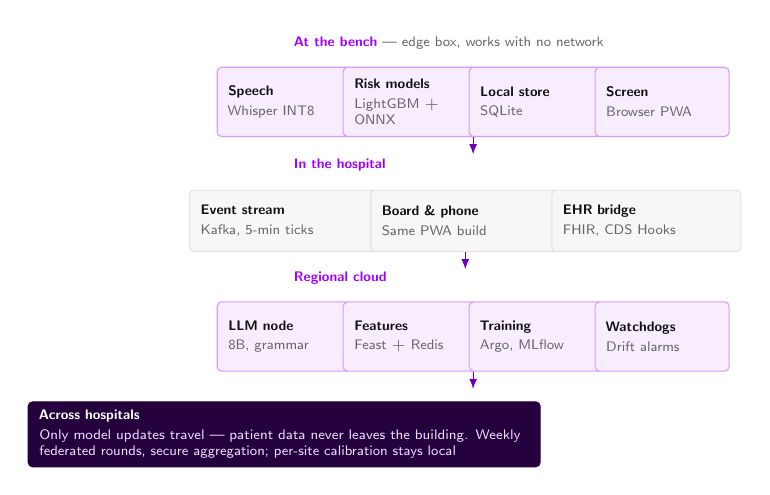
\begin{tikzpicture}[x=1cm,y=1cm,
  quad/.style={text width=1.42cm,anchor=north,minimum height=0.88cm,font=\sffamily\tiny},
  trip/.style={text width=2.12cm,anchor=north,minimum height=0.78cm}]
\node[lbl,anchor=west] (l1) at (0,0)
  {\textbf{\textcolor{AccPurple}{At the bench}} --- edge box, works with no network};
\node[bxa,quad] (sp) at (0,-0.30)      {\lyo{Speech}\sub{Whisper INT8}};
\node[bxa,quad] (rk) at (1.60,-0.30)   {\lyo{Risk models}\sub{LightGBM $+$ ONNX}};
\node[bxa,quad] (ls) at (3.20,-0.30)   {\lyo{Local store}\sub{SQLite}};
\node[bxa,quad] (sc) at (4.80,-0.30)   {\lyo{Screen}\sub{Browser PWA}};
\draw[flow] ($(sp.south)!0.5!(sc.south)+(0,0)$) -- ++(0,-0.22)
  node[coordinate,pos=1](midA){};

\node[lbl,anchor=west] (l2) at (0,-1.55)
  {\textbf{\textcolor{AccPurple}{In the hospital}}};
\node[bx,trip] (ev) at (0,-1.86)     {\lyo{Event stream}\sub{Kafka, 5-min ticks}};
\node[bx,trip] (bp) at (2.30,-1.86)  {\lyo{Board \& phone}\sub{Same PWA build}};
\node[bx,trip] (eh) at (4.60,-1.86)  {\lyo{EHR bridge}\sub{FHIR, CDS Hooks}};
\draw[flow] ($(ev.south)!0.5!(bp.south)+(1.15,0)$) -- ++(0,-0.22);

\node[lbl,anchor=west] (l3) at (0,-2.98)
  {\textbf{\textcolor{AccPurple}{Regional cloud}}};
\node[bxa,quad] (llm) at (0,-3.28)   {\lyo{LLM node}\sub{8B, grammar}};
\node[bxa,quad] (ft)  at (1.60,-3.28){\lyo{Features}\sub{Feast $+$ Redis}};
\node[bxa,quad] (tr)  at (3.20,-3.28){\lyo{Training}\sub{Argo, MLflow}};
\node[bxa,quad] (wd)  at (4.80,-3.28){\lyo{Watchdogs}\sub{Drift alarms}};
\draw[flow] ($(llm.south)!0.5!(wd.south)+(0,0)$) -- ++(0,-0.22);

\node[bxd,text width=6.22cm,anchor=north] (ac) at (0,-4.55)
  {\textbf{Across hospitals}\subw{Only model updates travel --- patient data never
   leaves the building. Weekly federated rounds, secure aggregation; per-site
   calibration stays local}};
\end{tikzpicture}
\caption{The technology stack, bench to federation. The bench and in-hospital
layers hold all patient data locally; only weight updates leave the building, into
the regional-cloud and cross-hospital layers below.}
\label{fig:stack}
\end{figure}

\begin{center}\footnotesize\sffamily
\begin{tabular}{@{}p{0.5cm}p{1.9cm}p{1.6cm}p{3.1cm}@{}}
\toprule
\rowcolor{AccPurple!10}
& \textbf{Setting} & \textbf{Hardware} & \textbf{Model path}\\
\midrule
\textbf{T1} & Metro tertiary / AIIMS-class & On-prem GPU & Full ASR + LLM;
  full ETHOS/CLMBR foundation model\\
\addlinespace[2pt]
\textbf{T2} & District, 50--200 beds & Edge GPU (Jetson-class) & Distilled INT8 path;
  lightweight encoder\\
\addlinespace[2pt]
\textbf{T3} & PHC / sub-district & CPU-only edge & Rule-based ATP fallback;
  no foundation model\\
\bottomrule
\end{tabular}
\end{center}

\vspace{3pt}
\textbf{Unit economics.} The target is \textbf{under Rs.\,5 per patient encounter},
achieved by a cascade: the GBDT head runs on 100\% of patients at millisecond cost,
while the LLM and foundation-model paths fire only on the $\sim$15\% flagged
ambiguous. Marginal cost falls as sites join the federated network, which keeps the
system reachable for district and government facilities rather than only for private
tertiary chains.

% ======================= 9. GOVERNANCE =======================
\section{Governance and Compliance}
\label{sec:gov}

MediPilot is Software as a Medical Device under CDSCO, \textbf{Class B or C}; we
design to Class C throughout as the conservative reading. CDSCO's draft
\textbf{Algorithm Change Protocol} (21 Oct 2025) [4] --- India's analogue to
the FDA/Health Canada/MHRA PCCP of Aug 2025 [5] --- provides the route for
retraining without full resubmission, and the federated update cycle
(\S\ref{sec:train}) is designed to fall inside it. Data governance, algorithmic
transparency, human oversight and independent audit follow ICMR's March 2023 ethical
guidelines [8].

\begin{tcolorbox}[mpbox,colframe=DeepPurple]
\textbf{The consent gap.} ABHA consent artifacts --- FHIR-based exchange across
\textbf{46.8 crore} ABHA IDs and 31 crore linked records as of Oct 2023
[1] --- \textbf{do not by default satisfy DPDP Act 2023 §6(1)}. ABDM
consent covers \emph{record access}; it does not cover the use of those records as
\emph{AI model input features}. MediPilot therefore issues a separate,
purpose-specific DPDP consent artifact per processing purpose. Ambient monitoring
carries its own consent, taken at registration and posted on visible signage.
\end{tcolorbox}

\vspace{3pt}
Every recommendation, every override with its stated reason, and every eventual
outcome is written to a cryptographically signed, append-only log serving three
consumers: medico-legal evidence, the Loop B training signal, and regulatory audit.

\subsection{Leakage lint --- the enforcement artifact}
The registry claim of \S\ref{sec:prior} is only credible if a build can fail because
of it. Each feature carries a registry entry, and CI rejects any training config whose
input set intersects the prohibited class:

\begin{tcolorbox}[mpcode]
feature: antibiotic\_order\_to\_first\_dose\\
\ \ downstream\_of\_suspicion: \textcolor{AccPurple}{true}\\
\ \ leakage\_class: \textcolor{AccPurple}{PROHIBITED}\\
\ \ permitted\_use: [outcome\_label, eval\_endpoint]\\[3pt]
\$ medipilot-lint train.yaml\\
\ \ \textcolor{AccPurple}{FAIL} \ 1 PROHIBITED feature in input\_features
\end{tcolorbox}

% ======================= 10. FAILURE MODES =======================
\section{Failure Modes}

\begin{center}\footnotesize\sffamily
\begin{tabular}{@{}p{1.85cm}p{5.5cm}@{}}
\toprule
\rowcolor{AccPurple!10}
\textbf{Failure} & \textbf{Mitigation}\\
\midrule
Missing data as the norm & Train-time modality dropout; the T0-only configuration is
an explicitly tested worst case\\
\addlinespace[2pt]
Atypical presenters & Phenotype clustering plus cost-matrix upweighting, treated as
the deadliest under-triage class\\
\addlinespace[2pt]
Power / network loss & Offline-first edge inference, UPS operation,
store-and-forward sync\\
\addlinespace[2pt]
Model service outage & Hard fallback to the frozen AIIMS-ATP red-flag rule card
[3]. The UI never shows a blank state\\
\addlinespace[2pt]
Pulse-oximeter bias & Normal SpO\textsubscript{2} carries no de-escalation authority;
Fitzpatrick-stratified pallor calibration\\
\addlinespace[2pt]
Adversarial gaming & Complaint-text distribution tracked against outcome correlation
as a drift signal, reviewed by clinical governance\\
\addlinespace[2pt]
Linguistic diversity & Code-mixed IndicWhisper ASR, multilingual IndicBERT,
per-language under-triage rate as a mandatory fairness metric\\
\bottomrule
\end{tabular}
\end{center}

% ======================= 11. ANTI-DECISIONS + IMPACT =======================
\section{Anti-Decisions, Impact, and Conclusion}

\textbf{What MediPilot must not become.} No virtual-nurse persona or avatar, which
manufactures false clinical authority. No spoken acuity level within patient earshot,
for dignity and panic reasons in shared waiting halls. No LLM-assigned severity,
which is structurally prohibited in L1 rather than merely discouraged. No autonomous
de-escalation, ever. And no chart-review labelling project --- outcome-derived labels
route around it entirely.

\textbf{Who this helps.} The single triage nurse under load gains a continuous
monitoring layer she cannot physically provide. The patient deteriorating in the
corridor is re-scored every five minutes rather than every time someone happens to
look. The district hospital without a certified emergency physician [2]
gains structured decision support grounded in the AIIMS-ATP foundation
[3].

\textbf{Go-to-market wedge.} The first shipped product is the
\emph{deterioration-while-waiting re-triage module} alone. It carries the highest
clinical value and the lowest regulatory exposure, because it never assigns an initial
acuity --- it only watches a queue a human already ordered. It requires near-zero
workflow change, and it generates the site-specific outcome data that every later
capability depends on.

\textbf{Moat.} A well-funded competitor can rebuild the technical stack in a year.
It cannot rebuild years of site-specific calibration and federated override history
across dozens of Indian EDs. Each new hospital improves the model for every other one
--- a compounding advantage structurally unavailable to a single-site or late entrant.

\textbf{Conclusion.} The waiting-room death is a systems failure with a specific
shape: one assessment, then silence. MediPilot's contribution is not a better score
but a better contract --- a machine that is allowed to raise an alarm on its own and
is never allowed to lower one, that abstains out loud when it does not know, and that
is evaluated on the patients it misses rather than on the average it gets right.

\vspace{6pt}
\noindent\parbox{\linewidth}{%
  \textcolor{AccPurple}{\rule{\linewidth}{1pt}}\\[3pt]
  \centering\sffamily\footnotesize
  \textcolor{AccPurple}{\bfseries Medi}{\bfseries Pilot} \ \textbullet\ \
  \textit{``Nobody waits unseen.''}\\[3pt]
  \textcolor{Border}{\rule{\linewidth}{0.5pt}}}

% ======================= REFERENCES =======================
\vspace{9pt}
{\sffamily\bfseries\small\color{NearBlack}REFERENCES}\par
\vspace{-1pt}\textcolor{AccPurple}{\rule{\linewidth}{1pt}}\par\vspace{2pt}

{\scriptsize
\begin{enumerate}[leftmargin=1.3em,itemsep=1.5pt]
\item ABDM (2023). \textit{Ayushman Bharat Digital Mission programme documentation}.
  MoHFW, Government of India.
\item Academic College of Emergency Experts (India) \& WHO Collaborating Centre for
  Emergency and Trauma, SEA (n.d.). \textit{Strategies to combat overcrowding at
  emergency departments across India}.
\item Aggarwal P.\ et al.\ (2020). AIIMS Triage Protocol (ATP) of a busy ED.
  \textit{J.\ Emerg.\ Trauma Shock} 13(2).
\item CDSCO (2025). \textit{Draft guidance on medical device software including
  algorithm change protocol for AI/ML software}, 21 Oct 2025.
\item FDA / Health Canada / MHRA (2025). \textit{Joint final guidance: predetermined
  change control plans for AI-enabled medical device software}, Aug 2025.
\item Haim L.\ et al.\ (2024). Evaluating LLM-assisted emergency triage: acuity
  assessments by GPT-4 versus medical experts. \textit{J.\ Clin.\ Nursing}.
\item HL7 International (n.d.). \textit{CDS Hooks specification}.
  \url{https://cds-hooks.org}
\item ICMR (2023). \textit{Ethical guidelines for application of AI in biomedical
  research and healthcare}, Mar 2023.
\item Kaiser Permanente Division of Research (n.d.). \textit{Evaluation of the
  Emergency Severity Index in US emergency departments for the rate of mistriage}.
\item \textit{Reliable generation of privacy-preserving synthetic EHR time series via
  diffusion models} (2024). \textit{JAMIA}.
\item Sjoding M.W.\ et al.\ (2020). Racial bias in pulse oximetry measurement.
  \textit{NEJM}; multicentre VA cohort, \textit{BMJ} (2022).
\item Wong A.\ et al.\ (2021). External validation of a widely implemented
  proprietary sepsis prediction model in hospitalized patients.
  \textit{JAMA Intern.\ Med.}
\item Xie F.\ et al.\ (2021). Benchmarking emergency department prediction models with
  machine learning and large public electronic health records.
  \textit{arXiv:2111.11017}.
\end{enumerate}
}

\vspace{8pt}
{\sffamily\bfseries\small\color{NearBlack}DESIGN COMMITMENTS AT A GLANCE}\par
\vspace{-1pt}\textcolor{AccPurple}{\rule{\linewidth}{1pt}}\par\vspace{3pt}

{\footnotesize\sffamily
\begin{tabular}{@{}p{1.85cm}p{5.5cm}@{}}
\toprule
\rowcolor{AccPurple!10}
\textbf{Commitment} & \textbf{Enforcing mechanism}\\
\midrule
Never de-escalates alone & Architectural constraint in L4 and Loop A, not a
configurable setting\\
\addlinespace[2pt]
Never learns clinician suspicion & \texttt{PROHIBITED} leakage class; CI build
failure (\S9.1)\\
\addlinespace[2pt]
Never assigns acuity by LLM & No production rule for acuity exists in the L1
output grammar\\
\addlinespace[2pt]
Never guesses silently & Conformal abstention gate; the card says so on the
$\sim$30\%$\rightarrow$$<$10\% it declines\\
\addlinespace[2pt]
Never trades safety for throughput & ED load reaches L4 only; it is excluded
from L2--L3 risk scoring\\
\addlinespace[2pt]
Never claims impact it cannot attribute & Stepped-wedge cluster randomisation, not
pre/post comparison\\
\bottomrule
\end{tabular}}

\vspace{7pt}
{\scriptsize\color{MedGray}\textbf{Note on format.} No style guidelines were issued
for this submission at the time of writing; the document follows standard technical
white-paper conventions and can be reformatted on request.}

\end{document}
